\section{Certifiability versus Payoff}
\label{sec:certify}

Section~\ref{sec:locality} measured potential under an oracle that knows each recorded observation. A deployed cache
has to decide from the query and the runtime alone, before it reuses anything. This section answers Q2. It
establishes which calls a cache can reuse without changing the observed result, and which of them it can recognize
in advance.

% Table 1 -- funnel (column width)
\begin{table}[htbp]
  \caption{Admission funnel over all 76,213 database calls: pooled shares of calls, isolated DB-execution time (a
  timeout counts at the 120\,s cap) and payload bytes. Gates are cumulative. The last two rows are the post-hoc E-eval
  (assumption-based) and B-eval (certified) subsets. They hold the calls of the static E and B rules whose replay is
  byte-identical to the recorded observation and stable across three replays. The oracle (potential) admits every call
  whose replay is equivalent to the recorded observation.}
  \label{tab:funnel}
  \small\setlength{\tabcolsep}{3pt}
  \begin{tabular}{@{}L{3.15cm}rrrr@{}}
\toprule
Gate (cumulative) & Calls & \% calls & \% DB time & \% bytes \\
\midrule
Successful replay & 71,582 & 93.9 & 94.7 & 100.0 \\
Equivalent to recorded observation (oracle) & 70,173 & 92.1 & 94.2 & 98.8 \\
Byte-identical, stable in 3 replays & 66,556 & 87.3 & 93.9 & 98.8 \\
E-eval subset (static E, post hoc) & 66,263 & 86.9 & 93.6 & 98.7 \\
B-eval subset (static B, post hoc) & 5,695 & 7.5 & 9.4 & 0.023 \\
\bottomrule
\end{tabular}

\end{table}

% Fig. 3 -- admission per engine and the verdicts of the static Contract B rule (column width, Section 5)
\begin{figure}[htbp]
  \centering
  \subcaptionbox{The funnel of Table~\ref{tab:funnel} per engine\label{fig:funnelengine}}{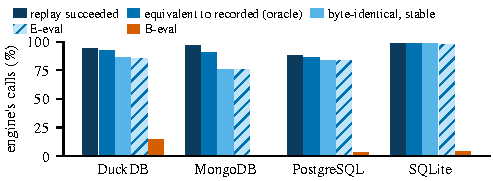
\includegraphics[width=\columnwidth]{figures/fig3a_funnel_engine}}
  \subcaptionbox{Verdicts of the static Contract B rule\label{fig:verdicts}}{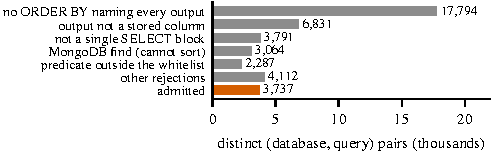
\includegraphics[width=\columnwidth]{figures/fig3b_b_verdicts}}
  \caption{Admission by engine and by rule. (a) Share of each engine's calls that passes each cumulative gate of Table~\ref{tab:funnel}. It covers the 76,141 calls with a replay outcome, and Table~\ref{tab:workload} gives the totals.
  MongoDB's B-eval subset, two calls, is too small to see. (b) Verdict of the static Contract B rule on each of the 41,616 distinct (database, query) pairs. Bars show rejection reasons and the admitted pairs.}
  \label{fig:certify}
  \Description{Two panels. Top: grouped bars per engine showing that most calls of every engine pass the replay, equivalence, byte-identity and E-eval gates, while the B-eval subset is a small share. Bottom: horizontal bars of the number of distinct (database, query) pairs per verdict of the static Contract B rule. The longest bar is the rejection for lacking an ORDER BY that names every output.}
\end{figure}


\subsection{Admission Funnel}
\label{sec:funnel}

Table~\ref{tab:funnel} follows all 76,213 calls through cumulative gates, and Figure~\ref{fig:funnelengine} splits
them by engine. Replay succeeds for 93.9\% of the calls. In all, 92.1\% of the calls reproduce the recorded
observation up to normalization, with 94.2\% of the DB time and 98.8\% of the bytes. A further gate keeps the 87.3\%
that reproduce it byte for byte and stably over three replays. Of the 4,977 byte mismatches between the original
runs and the replay, 2,290 are row-order differences. These comprise 1,743 of 2,263 in DuckDB, which the original
runs used multi-threaded, and 547 of 953 in PostgreSQL. Object identifiers reassigned at load time explain 1,299 of
the 1,757 MongoDB mismatches. After these gates, the static Contract E rule leaves 86.9\% of the calls, the E-eval
subset. Contract B leaves 7.5\%, the B-eval subset.

Before any replay, Contract B admits 5,697 calls (7.5\%) with 9.4\% of the DB time and 0.023\% of the payload bytes.
Every one of these calls completed in each of its replays. For 5,695 of them the original trace records a result,
and every replay is byte-identical to it. This holds although the original runtime ran DuckDB with several threads.
These calls form the B-eval subset, and the remaining 2 have no recorded result. Figure~\ref{fig:verdicts} gives the
rule's verdict on the 41,616 distinct (database, query) pairs. The most frequent rejection, 17,794 pairs, is
\emph{unordered result}: the query is not a one-row aggregate and has no \texttt{ORDER BY} that names every output.
A further 6,831 pairs output something other than stored columns, such as \texttt{SELECT *} or computed values. The
rule accepts 3,507 pairs that return one row of counts and extrema and 228 whose \texttt{ORDER BY} names every
output. It also accepts 2 MongoDB lookups by object identifier.

The gap does not depend on how the rule is written. Of the successful calls, 58.7\% return at least two distinct
rows from a statement without a top-level \texttt{ORDER BY}. They carry 65.0\% of the DB time and 79.2\% of the
bytes of the successful calls. The engines leave the order of such rows unspecified
\cite{postgres2026order,sqlite2026select,mongodb2026sort}, so two correct executions can serialize them differently.
No rule that guarantees the bytes across plans can admit these calls while the tool serializes rows in the order the
engine returns. This holds whatever the rule knows about the schema or the data.

\subsection{Payoff beyond the Certificate}
\label{sec:gap}

Most of the cross-attempt payoff lies outside Contract B. Of the cross-attempt repeats of Section~\ref{sec:scope},
the static B rule admits 6.4\% of the calls, 12.2\% of the DB time and 0.00005\% of the bytes. Its B-eval subset
holds the same shares at this precision. The static E rule admits 99.5\% of the calls and essentially all of the DB
time and bytes. The E-eval subset holds 93.2\% of the calls, 99.8\% of the DB time and essentially all of the bytes
(Figure~\ref{fig:tiers}). Restricting reuse to what Contract B certifies thus forgoes 87.8\% of the reusable DB time
and nearly all of the reusable bytes. A less conservative certificate with the same across-plan guarantee cannot
close the gap. We exclude the successful calls that return at least two distinct rows without a top-level
\texttt{ORDER BY}. The remaining calls are a conservative upper bound for such a rule. They carry 27.1\% of the
reusable DB time and 17.2\% of the reusable bytes. Within each tier's own calls, S2 saves 6.4\% of the median task's
DB-execution time on the B-eval subset (certified) at $N=8$ with an unbounded budget. It saves 24.5\% on the E-eval
subset (assumption-based) and 24.1\% under the oracle (potential).

\subsection{Runtime Qualification}
\label{sec:pinning}

Of the 71,582 calls whose replay succeeded, static Contract E admits 71,275, which cover 37,542 distinct queries.
Inside the pinned runtime every one of them replayed byte-identically three times. Against the observation recorded
in the original runtime, 7.0\% of them differ. These calls carry 0.8\% of their DB time and 1.2\% of their bytes,
and 8.3\% of the repeated calls a cache would serve. Row order alone accounts for 3.2 points and different values
for 2.2. Spilled results whose recorded preview differs account for 1.5, and calls with an error or no result in the
original trace for 0.07. After normalization, 5.1 of the 7.0 points are equivalent. By engine, DuckDB contributes 3.2
points, MongoDB 2.5, PostgreSQL 1.4 and SQLite 0.02. For the calls that Contract E admits and Contract B does not
certify, byte stability is thus an empirical property of the qualified pinned runtime. One pinned runtime reproduced
every admitted result it executed, while two runtimes disagreed on 7.0\% of them. The E-eval numbers are therefore
the payoff under a pinned runtime that was qualified offline. Qualification replays every query three times and
compares it with the recorded observation. The post-hoc gates do not produce that payoff. A cache can apply the
static E rule online and admit every successful call of that rule. S2 then saves 23.8\% of the median task's
DB-execution time at $N=8$, against 24.5\% on the E-eval subset. S3 writes 0.45$\times$ the bytes of S2 in both
cases. The rule also holds on queries it was not written against. The four leaderboard harnesses of
Section~\ref{sec:xharness} issued 8,811 distinct queries whose replay succeeded, 8,382 of them in no DAB trajectory.
Static E, in a code snapshot taken before they were replayed, admits 8,592 of them. Every admitted query returned
the same bytes in three replays. All 27 calls whose replays differed belong to queries that the rule rejects.

\subsection{Reuse-Key Sensitivity}
\label{sec:keys}

Exact text is a conservative key. On the E-eval subset, normalizing whitespace and comments raises the median S2 DB-execution saving from 16.6\% to 17.5\% at $N=4$. At $N=8$ it raises the saving from 24.5\% to 25.2\%. A canonical abstract syntax
tree adds 3.6 and 5.2 points (20.1\% and 29.8\%). An oracle that matches equal results reaches 33.7\% and 48.0\%, or
27.0\% and 37.3\% when empty and single-row results are excluded. It needs the result to decide, so it is a bound,
not a cache.
